\documentclass{book}
\usepackage{../asy_sty/asy_tut}

% For 3D PRC asymptote
% See: https://github.com/vectorgraphics/asymptote/blob/master/doc/externalprc.tex
% Compile .asy files with asy -inlineimage <fn>
\RequirePackage{asymptote}
\def\asydir{chapter4/asy}
\graphicspath{ {asy/} {chapter4/asy/} }
% uncomment for 3D graphics: 
\input chapter4/asy/vectors.pre
\input chapter4/asy/planes.pre
\input chapter4/asy/washer.pre
\usepackage[bigfiles]{media9}


\includeonly{
  cover/cover,
  preface/preface,
  chapter1/chapter1,
  chapter2/chapter2,
  chapter3/chapter3,
  chapter4/chapter4,
  appendix/appendix
}

\begin{document}
\frontmatter
\newcommand{\includefiledir}{cover}
% !TeX root = ../exam-zh-doc.tex

\begin{abstract}
  本项目提供了一个中国高考试卷样式的 \LaTeX 模板,旨在帮助中小学教师更方便地使用 \LaTeX。模板具有以下特性:
  
  \begin{enumerate}
    \item 样式与内容尽可能分离;
    \item 选择题选项可以自动排版成合适的列数;
    \item 通过用户接口可以方便更改密封线样式;
    \item 在 Windows, macOS 和 Linux 跨平台编译。
  \end{enumerate}
\end{abstract}


\begin{tikzpicture}[remember picture, overlay]
  \node[opacity = 0.1,rotate = 30] at ([shift={(0,0)}]current page text area.center){
    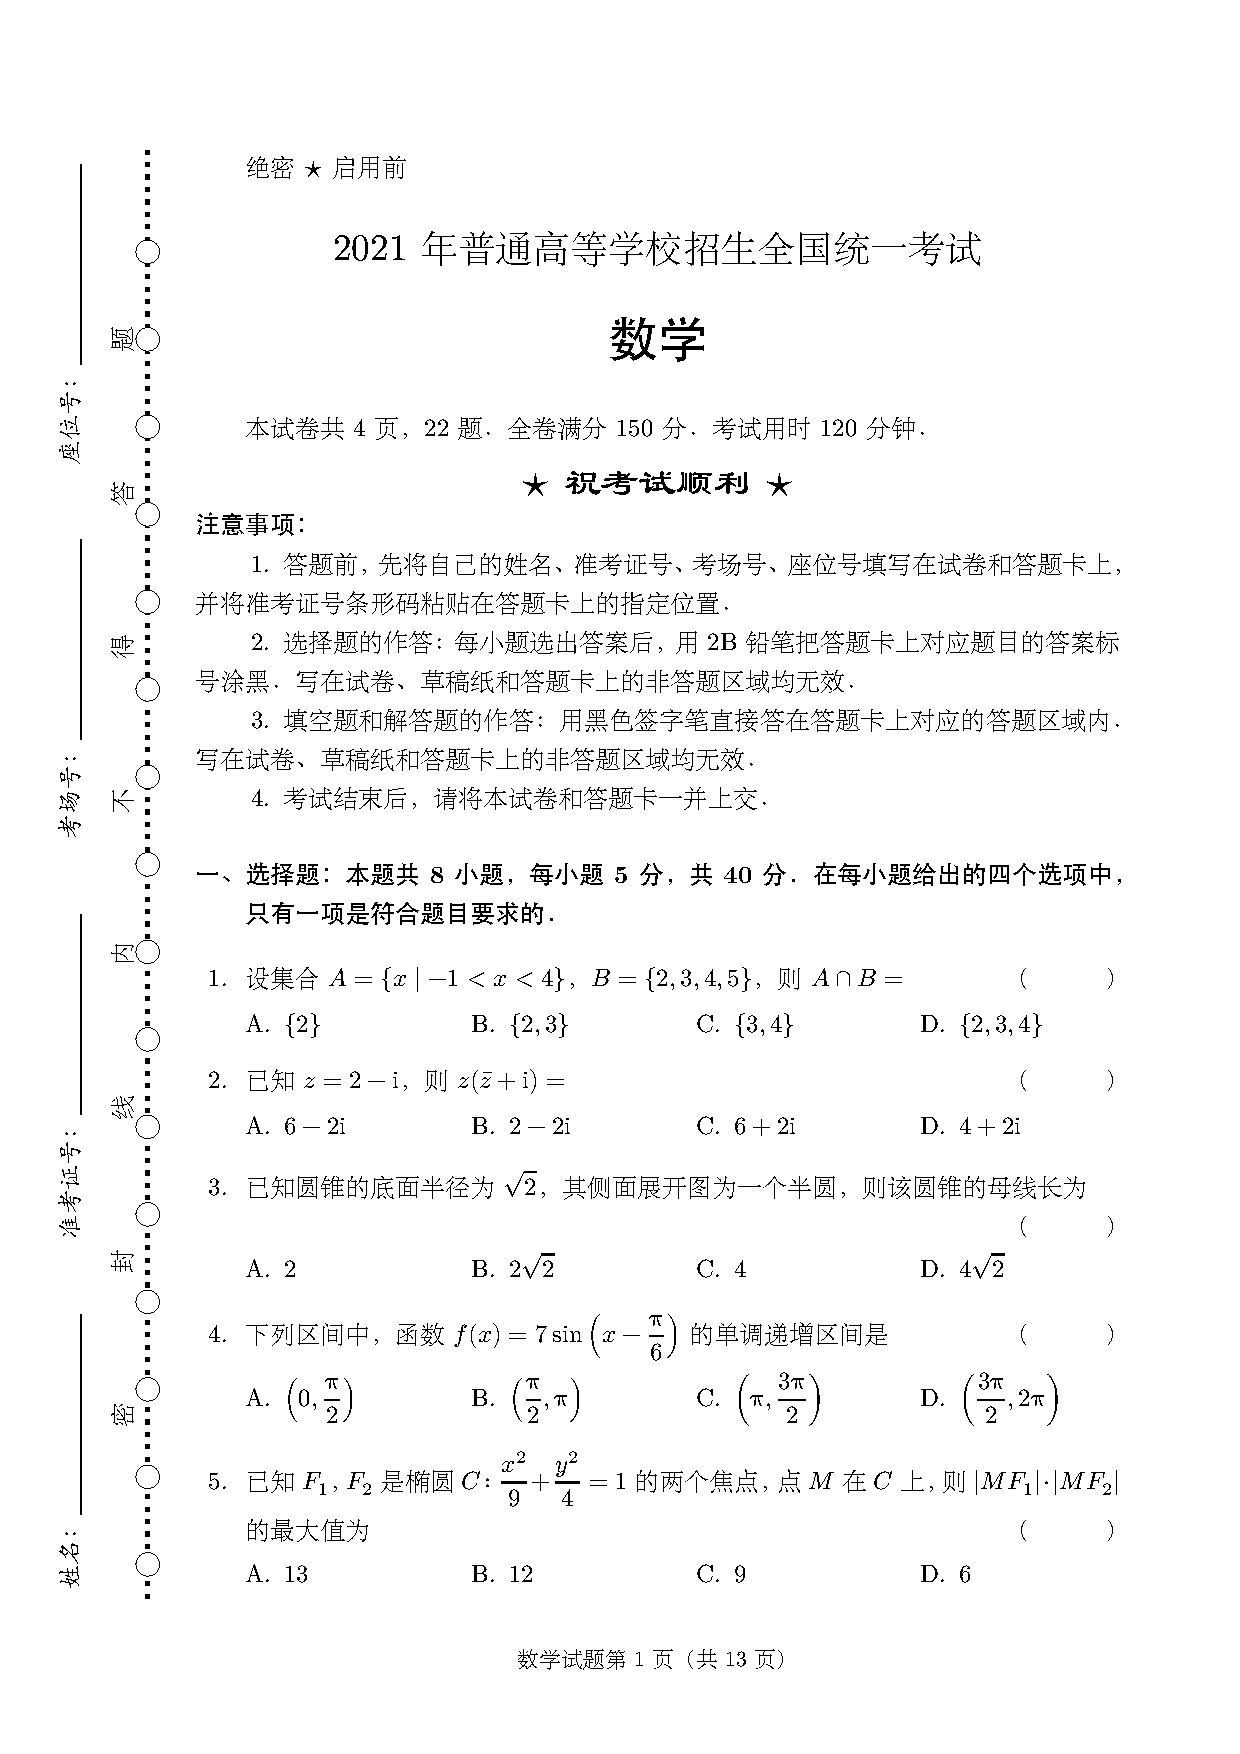
\includegraphics[width=23cm]{firstpage.pdf}
  };
\end{tikzpicture}
\thispagestyle{plain}
\clearpage
\renewcommand{\includefiledir}{preface}
% !TeX root = ../install-latex-guide-zh-cn.tex

\chapter*{前言}

以``啸行''名义加入 QQ 群 91940767、478023327 和 640633524 后,
经常有群友咨询如何安装 \LaTeX.
实际上,
用户安装的是 \LaTeX{} 的\textbf{发行版}和相关的\textbf{编辑器}.
本文将介绍在\textbf{不存在其他 \LaTeX{} 发行版 (如 C\TeX{} 套装) 的前提下},
在 Windows 11、Ubuntu 20.04 和 macOS 系统中安装
\TeX{}~Live (macOS 中介绍 Mac\TeX)、升级宏包、编译简易文档等相关操作,
并多以介绍命令行操作为主.
有关 MiK\TeX{} 的安装,
可以参考 \href{https://camusecao.top/2021-06-16/MiKTeX/}{MiK\TeX{} 的基本使用}.

本文还将简要介绍几款常见编辑器的使用方法,
其他编辑器如 \href{https://code.visualstudio.com/}{VS Code},
\href{https://www.vim.org/}{Vim},
用户可自行了解它们的使用方法.
鉴于 WSL 较为特殊,
本手册提供了一份 VS Code 配合
\href{https://marketplace.visualstudio.com/items?itemName=James-Yu.latex-workshop}{LaTeX Workshop}
的自用配置单,
仅供参考.

除在本地安装 \LaTeX{} 发行版和编辑器之外,
本文还额外补充两款在线的 \LaTeX 平台,
即 \href{http://www.overleaf.com}{Overleaf} 和 \href{https://www.texpage.com/}{TeXPage} 的相关内容.

本文所涉及到的代码需结合上下文说明, 不能简单地复制粘贴. 红色文字都是可点的超链接, 可直接跳转.
\menu{菜单} 表示软件菜单. \keys{k} 表示键盘按键.
建议用户阅读 \href{https://www.tug.org/texlive/doc/texlive-en/texlive-en.pdf}{texlive-en}
和 \href{http://mirrors.ctan.org/info/lshort/chinese/lshort-zh-cn.pdf}{lshort-zh-cn}
以更全面地了解基础内容.

必须声明的是,
即便你已经通读本手册和上面提到的两本书,
有很大概率还会碰到很多问题.
这时我希望用户可以按照正确方式提问,
例如提供\textbf{最小工作示例},
并在论坛上面留下你的问题和相应解答以方便后来者.

本文大部分内容是个人过去一段时间的使用总结, 其中难免有不甚合理或晦涩难懂的部分. 
若用户在阅读本文档的过程中有任何意见和建议,
请发\href{mailto:ranwang.osbert@outlook.com}{邮件}或在
\href{https://github.com/OsbertWang/install-latex-guide-zh-cn/}{GitHub} 中提 issue.
本文另在\href{https://gitee.com/OsbertWang/install-latex-guide-zh-cn}{码云}%
有备份,
并于 2020 年 7 月提交至 CTAN.


本手册发布后,
\href{https://github.com/EthanDeng}{Dongsheng Deng},
\href{https://github.com/muzimuzhi}{muzimuzhi},
\href{https://github.com/stone-zeng}{Xiangdong Zeng},
\href{https://github.com/tauyoungsama}{tauyoung}
对本手册提出了很好的建议, 并提供了帮助,
其中, 有关 macOS 的内容最初由 Xiangdong Zeng 草拟完成,
而后 Dongsheng Deng 进行了补充,
最近一次更新则由 tauyoung 提供.
在此一并感谢.

\mainmatter
\renewcommand{\includefiledir}{chapter1}
% Chapter 1 from Asymptote tutorial Jim Hefferon
\chapter{A first graphic}
Making an \Asy{} input file is like making a \LaTeX{} input file,
so you already have a feel for the basics.
To start, 
use your favorite editor to open a file \path{asy/unit_circle.asy}.
\begin{minted}{Bash}
jim@millstone:~/Documents/asy_tut/src$ cd asy
jim@millstone:~/Documents/asy_tut/src/asy$ emacs unit_circle.asy  
\end{minted}
Type this text into the file and save it, or
copy it from this document's online source.
\begin{center}
  \inputminted{Asymptote}{chapter1/asy/unit_circle.asy}
\end{center}
Get the output file \path{unit_circle.pdf} by running \Asy{} on the source.
\begin{minted}{Bash}
jim@millstone:~/Documents/asy_tut/src/asy$ asy unit_circle  
\end{minted} 
%$ Make auctex recognize end of "math"
You can see the result in any PDF viewer.
\begin{center}
  \includegraphics{chapter1/asy/unit_circle.pdf}
\end{center}




\section{What do we have here?}
The input \path{unit_circle.asy} illustrates a number of things.
Globally, it shows that you must declare variables such as line~12's
\mintinline{Asymptote}{theta}, that
commands end with a semicolon,
and that comments are preceded by a double slash, 
\mintinline{Asymptote}{//}.

Locally, line 2's \mintinline{Asymptote}{settings.outformat}
variable fixes the format of output files to PDF so we needn't remember 
each time to do that from the command line.
Line~4's \mintinline{Asymptote}{import}
is like a \LaTeX{} \mintinline{TeX}{\usepackage{...}} in that
it gives us access to a module, a collection of related commands and data.
In this case it
gives us commands to make plots.
In this drawing we only use its axis-making commands 
but the second chapter has more about plots.

In line~6 the \mintinline{Asymptote}{unitsize(1.5cm)} command means that
if we describe a point $(x,y)$ then \Asy{} will interpret it as the
location $x\cdot 1.5\text{\,cm}$ and $y\cdot 1.5\text{\,cm}$ from the origin.
 
Line~9 is self-explanatory.
Lines~12 through~15 draw the line segment from the origin to the 
point labeled $(\cos\theta,\sin\theta)$.
(On line~15, in addition to drawing the dot, \Asy{} labels it and
the \mintinline{Asymptote}{E} puts that label east of the dot.)
% Note that if after seeing the drawing we decide to adjust the angle
% then we just need to change one number, on line~12. 

Finally, lines 18 and~19 draw the axes.
These commands have many options, most of which we did not use here,
and we will see more of them later.

One more thing.
\Asy{} gets the point label $(\cos\theta,\sin\theta)$ and the axis labels
by putting the given strings in a small file,
running \LaTeX{} on it, and then extracting the result back into the
output graphic.
So your labels have access to all of \LaTeX's capabilities.  





\section{Adjustments}
After you get a graphic draft there are always some tweaks.

First, here the axis labels are too big.
We will replace \mintinline{Asymptote}{"$x$"}
with \mintinline{Asymptote}{"\scriptsize $x$"}.
(We could instead omit the label by deleting the entire
string and the comma after it,
which illustrates that commands
such as \mintinline{Asymptote}{"xaxis(..)"}
can have a variable number of arguments.
While you are working you may want to have open the \Asy{} reference
for a list of the options.)

Second, the dot showing the generic point on the unit circle is too big.
In the revised source below we've adjusted the size by inserting
\mintinline{Asymptote}{dotfactor = 4} in line~22
(the default factor is $6$).

Finally, the $(\cos\theta,\sin\theta)$ label is in a different font than
the other mathematics in this overview.
We want that \Asy, when making the small \LaTeX{} document to create the
in-graphic text,
will use the same font setup as the main \path{.tex} file.
So below we added a 
\mintinline{Asymptote}{texpreamble("..")};~the 
string is long so for readability we've spread it across multiple lines.
\begin{center}
  \inputminted{Asymptote}{chapter1/asy/unit_circle_after.asy}
\end{center}
\begin{center}
  \includegraphics{chapter1/asy/unit_circle_after.pdf}
\end{center}



\section{Include the graphic in a \LaTeX{} file}
Open a new \LaTeX{} file \path{main.tex}. 
\begin{minted}{Bash}
jim@millstone:~/Documents/asy_tut/src$ emacs main.tex  
\end{minted} 
Enter this text
or copy it from this document's source.
\begin{center}
  \inputminted{TeX}{chapter1/main.tex}
\end{center} 
This document shows two ways to include the graphic.
Line~11 is straightforward because
after you've iterated through some adjustments to the figure then you   
use \LaTeX's standard \mintinline{TeX}{\includegraphics{..}}.
The other way, commented out, 
uses the \mintinline{TeX}{asymptote} \LaTeX{} package
to include the \Asy{} source file with 
\mintinline{TeX}{\asyinclude{..}}.
In this approach, getting the graphic is a three step process, where 
you run ``\mintinline{Bash}{pdflatex main}'' (of course
you can instead use ``\mintinline{Bash}{xelatex main}'' or 
``\mintinline{Bash}{lualatex main}''), then you go into
the \path{asy/} subdirectory and run 
``\mintinline{Bash}{asy <latex-filename>-1}''
(here, ``\mintinline{Bash}{asy main-1}''), then go back to the
\LaTeX{} file's directory and run ``\mintinline{Bash}{pdflatex main}'' once more.
In either case here is the one-page output.
\begin{center}
  \framebox{\includegraphics[page=1,scale=0.325,trim=0.25in 5.9in 0.25in 0.25in]{chapter1/main.pdf}}
\end{center}



\renewcommand{\includefiledir}{chapter2}
% Chapter 2 from Asymptote tutorial Jim Hefferon
\chapter{Plots}
We will draw this function.
\begin{equation*}
  f(x)=x+\frac{1}{x-1}
\end{equation*}
It goes infinite at $x=1$ so
we can't ask \Asy{} to plot all $x$'s. 
We will instead plot the $x$'s where the associated $y$'s 
are between $-5$ and~$5$. 
To find these
we can use a computer algebra system such as \textit{Sage} to solve
$5=x+1/(x-1)$ and $-5=x+1/(x-1)$.
\begin{minted}{Python}
sage: x = var('x')
sage: solve( [5==x+(1/(x-1))], x )
[x == -sqrt(3) + 3, x == sqrt(3) + 3]
sage: solve( [-5==x+(1/(x-1))], x )
[x == -2*sqrt(2) - 2, x == 2*sqrt(2) - 2]
sage: round(-sqrt(3) + 3, ndigits=3)
1.268
sage: round(2*sqrt(2) - 2, ndigits=3)
0.828
\end{minted}
That leads to this source file \path{asy/plot.asy}.
\begin{center}
  \inputminted{Asymptote}{chapter2/asy/plot.asy}
\end{center}
Here is the resulting plot.
\begin{center}
  \includegraphics{chapter2/asy/plot.pdf}
\end{center}



\section{Adjustments}
As earlier, on seeing the draft graphic we make some tweaks, 
which helps give a sense of some available options,
leading to the 
source \path{asy/plot_after.asy} below.

The axes go through the two $0$'s
and the vertical asymptote passes through the~$1$.
We can change the \mintinline{Asymptote}{xaxis(..)}
command to say \mintinline{Asymptote}{RightTicks(Step=1, OmitTick(0,1))},
and similarly change \mintinline{Asymptote}{yaxis(..)}.

Although we limited the output range to between $y=-5$ and~$5$, 
the plot is still so tall that it is hard to fit on a page or slide.
We make the $y$~unit height be half of the $x$ unit width by adding this command
\begin{minted}{Asymptote}
scale(Linear, Linear(0.5))
\end{minted}
(\mintinline{Asymptote}{Linear} is in contrast with a 
\mintinline{Asymptote}{Logarithmic} scale).
The axes and graph now come out rescaled but
we must also adjust the location
of points, the ones defining the vertical asymptote line, using for example 
line~26's \mintinline{Asymptote}{Scale((1,ymin))}.

That tweak of the $y$~axis causes its tick labels to be scrunched together,
so we arrange that \Asy{} labels only every fifth tick
(the labeled ones are called major ticks and the others are minor ticks). 
\begin{minted}{Asymptote}
  yaxis(ymin=ymin-0.4, ymax=ymax+0.4,
      LeftTicks(Step=5, step=1, OmitTick(0), Size=3pt, size=2pt),
      Arrows(TeXHead));
\end{minted}
That command also sets the length of these major and minor ticks.

Here is \path{asy/plot_after.asy}. 
An explanation of line~3 is in the next section.
\begin{center}
  \inputminted{Asymptote}{chapter2/asy/plot_after.asy}
\end{center}
Here is the output.
\begin{center}
  \includegraphics{chapter2/asy/plot_after.pdf}
\end{center}



\section{Defaults}
Rather than copy and paste elements common across graphics 
such as the font commands or colors,
we can put them in a separate file and import them,
as in the prior source's line~3.
The source of that file, \path{jh.asy}, is in the Appendix.
(About the
\mintinline{Asymptote}{"../../../asy/"} 
directory stuff:~usually we set up \Asy{} with a directory for common files
and then just say \mintinline{Asymptote}{import jh}.
But for this document we want that a user can compile without setup
so the relative path is in the source.)



\section{Ticks}
With plot ticks you often want something other
than the default.
We won't cover all of the options but there are a couple of things we have
not yet seen that are especially useful.

On a trigonometric graph
\begin{center}
  \includegraphics{chapter2/asy/cos.pdf}
\end{center}
you don't want the $x$~axis to say $1$, $2$, etc.,
you want $\pi/2$, $\pi$, etc.
You also don't want ``$3.14$,'' you want ``$\pi$.''
This illustrates explicit ticks, on lines 19 and~21.
\begin{center}
  \inputminted{Asymptote}{chapter2/asy/cos.asy}
\end{center}
Note line~25's \mintinline{Asymptote}{NW}, which prints
the $3\pi/2$ northwest of its tick. 

Our other tick example has a graph paper effect, 
with lines  in a light color extending across the graph.
(I sometimes use this for lectures; here, 
to estimate by eye that at $y=2$ the slope of the tangent line 
is~$2$.)
\begin{center}
  \includegraphics{chapter2/asy/exponential.pdf}
\end{center}

The source has a number of interesting features.
\begin{center}
  \inputminted{Asymptote}{chapter2/asy/exponential.asy}
\end{center}
The graph paper effect is due to the input in lines 26 through~46.
The horizontal lines are a little clearer so we will cover them.
They are created by the \mintinline{Asymptote}{yaxis(..)} commands
in lines 39--46.
These two vertical axes, one on the left and one on the right, 
are drawn with a \mintinline{Asymptote}{nullpen} so we don't see 
vertical black lines at \mintinline{Asymptote}{xmin-0.2}
and \mintinline{Asymptote}{xmax+0.2}.
What we do see are
the ticks for those axes,
extending back and forth between them in the color given by 
\mintinline{Asymptote}{GRAPHPAPERPEN}, because of 
the \mintinline{Asymptote}{extend=true}.
These ticks have a null label because of the 
\LaTeX{} comment character~\mintinline{Asymptote}{"%"}.
The $y$~axis on the left produces the horizontal 
graph paper marks between
$x=\text{\mintinline{Asymptote}{xmin-0.2}}$ and
$x=0$, while the one on the right generates the marks 
from $x=0$ to $x=\text{\mintinline{Asymptote}{xmax+0.2}}$.
(The $x=0$ comes from the $y$~axis in lines 52--54.)

The commands from line~49 to the end produce the axes shown in black.
% Note that \mintinline{Asymptote}{yaxis(..)} produces only one arrow.

This is a long file but we will discuss a few fine points.
One is that the $(\ln(2),2)$ label has a white background
obscuring some of the graph paper lines, from the
\mintinline{Asymptote}{Label("$(\ln(2),2)$",filltype=Fill(white))}
command.
Another is that the 300 in line~19's
\mintinline{Asymptote}{f = graph(fcn, xmin, xmax, n=300)}
is there because \Asy{} draws the graph by connecting dots that
evaluate 
\mintinline{Asymptote}{fcn}
at a finite number of points, and the default was too small so that
the graphic had visible jaggies.

Finally, lines 18 and~19 as well as lines 27 and~28 make clear that
essential to understanding \Asy{} is understanding the ideas of  
\mintinline{Asymptote}{path}
and
\mintinline{Asymptote}{pen}.
That's the next chapter.

\renewcommand{\includefiledir}{chapter3}
% Chapter 3 from Asymptote tutorial Jim Hefferon
\chapter{Paths and pens}

\section{Paths}
This plots a function that is generic in that it isn't 
derived from a simple expression such as $\cos x$ or $x+(1/(x-1))$.
We will use it for the classic Calculus 
lesson
illustrating that
the curve is locally well-approximated by the line,
by zooming in on a point of tangency.
\begin{center}
  \includegraphics{chapter3/asy/zoom.pdf}
\end{center}
Here is the source of that graphic.
\begin{center}
  \inputminted{Asymptote}{chapter3/asy/zoom.asy}
\end{center}
Line~7's \mintinline{Asymptote}{generic_fcn_plot} is a 
\mintinline{Asymptote}{path}.
It joins some points 
with smooth curves, using the \mintinline{Asymptote}{..} operator.
(I often use this path
so I included a copy in \path{jh.asy}
as \mintinline{Asymptote}{GENERIC_FCN_PLOT}.)
Earlier, when we drew a vertical asymptote line we instead connected two
points with a \mintinline{Asymptote}{--} operator, which gives a line segment.
There are other connectors but these two are the most common.

In line~17, \Asy's 
\mintinline{Asymptote}{dir(..)} command gives the direction of the
tangent line as a unit vector.
The two lines after that produce its graph.
As part of this, line~18 uses that \mintinline{Asymptote}{d.y} is the second
component of the pair \mintinline{Asymptote}{d} 
and \mintinline{Asymptote}{d.x} is its first component,
so the tangent line's slope is the ratio 
\mintinline{Asymptote}{d.y/d.x}.

As to line~15's \mintinline{Asymptote}{c_time = times(f, c)[0]}, 
\Asy{} joins the points with piecewise cubic Bézier curves,
just as \MF{} and \MP{} do. 
These curves are
parametrized by a variable called `time'.
By definition, the initial point $(0,-0.25)$ is at time~$0$, the next point 
$(1,0.35)$ is at time~$1$, etc.
(To forestall any confusion:~the time has nothing to do with the
first coordinate, it comes from when the point is specified in the
path.)
Intermediate points have intermediate times.
This illustrates, showing some times.
\begin{center}
  \includegraphics{chapter3/asy/zoom_times.pdf}
\end{center}
The \mintinline{Asymptote}{times(..)} command returns an array of times
where the path intersects the vertical line 
$x=\text{\mintinline{Asymptote}{c}}$.
We extract the first one (in this case the only one) with the 
\mintinline{Asymptote}{[0]}.
Then line~16's \mintinline{Asymptote}{c_point = point(f,c_time)} returns
that point as a \mintinline{Asymptote}{pair}.
(Incidentally, the time points need not be evenly spaced on a curve, meaning that
there may be a different arc length between $t=2.0$ and~$2.5$ than there is 
between $t=2.5$ and~$3.0$.)

The source for the prior graphic shows two useful aspects of
\Asy{} that are new.
\begin{center}
  \inputminted{Asymptote}{chapter3/asy/zoom_times.asy}
\end{center}
The first of those is in line~19.
The \mintinline{Asymptote}{format("$%0.02f$",t)} 
turns the floating point number~$t$ into the string used in the label.

The other is in lines~17 through~20, where the code has an iteration.
One strength of \Asy{} is that it is a standard programming language,
with clean constructs that are like those you use in other languages
in your daily work.
This iteration is over an array but an integer iteration
\mintinline{Asymptote}{for(int i=0; i<4; ++i)}
is in the next example.
 
That next example shows zooming in on the
point of tangency in four steps.
Here's the output.
\begin{center}
  \hspace{2em}%
  \vcenteredhbox{\includegraphics{chapter3/asy/zoom_iterate000.pdf}}%
  \hspace{1em plus 1fill}%
  \vcenteredhbox{\includegraphics{chapter3/asy/zoom_iterate001.pdf}}%
  \hspace{1em plus 1fill}%
  \vcenteredhbox{\includegraphics{chapter3/asy/zoom_iterate002.pdf}}%
  \hspace{1em plus 1fill}%
  \vcenteredhbox{\includegraphics{chapter3/asy/zoom_iterate003.pdf}}%
  \hspace*{2em}%
\end{center}

The source \path{asy/zoom_iterate.asy}
is more complex than the others that we have seen.
One reason is that this one file produces four pictures, 
so that we needn't maintain
four separate \path{.asy} files with lots of overlap.
The four output files are produced in the loop between lines~17 and~47.
Line~18 creates a new 
\mintinline{Asymptote}{picture}
and line~46 outputs it.
The files are named 
\path{zoom_iterate000.pdf} \ldots{} \path{zoom_iterate003.pdf};~the 
form of that name is given by the string
\mintinline{Asymptote}{OUTPUT_FN}.
\begin{center}
  \inputminted{Asymptote}{chapter3/asy/zoom_iterate.asy}
\end{center}

Besides using a single input to create multiple output files,
there are two other things that are new here.
One is line~19's
\mintinline{Asymptote}{size(pic, 3cm, 0)}.
This makes each output graphic be three centimeters wide and as tall as
required, setting the size of the $x$ and~$y$ units as needed to 
get that width.
The result is a zooming-in on successively shorter intervals of the $x$~axis.

The other new thing 
is that rescaling the units to make the
entire figure three centimeters wide
would put the plotted function very far above the
$x$~axis.
So we have moved the function down near the axis.
This transformation applies not just to the function but also to the tangent
line and to the point $(c,f(c))$, so we have broken this
transformation out as a separate thing,
in line~32.   
%\mintinline{Asymptote}{transform f_trans = shift(0,0.5*delta)*shift(0,-1*c_point.y)}.
Transformations are applied with the star operator, 
as on lines~33, 34, and~36.

In the next section we will see one more thing about paths, 
that if a path is closed then we can fill it.
 




\section{Pens}
When you draw something you need  to specify some properties, such as its color
or thickness if you are drawing a curve, or the font if you are
writing text.
\Asy{} binds those properties together as a 
\mintinline{Asymptote}{pen}. 

This source gives a picture showing the area computed with $\int_{a}^{b}f(x)\,dx$.
\begin{center}
  \inputminted{Asymptote}{chapter3/asy/integral.asy}
\end{center}
Here is the resulting graphic.
\begin{center}
  \includegraphics{chapter3/asy/integral.pdf}
\end{center}
The    
\mintinline{Asymptote}{buildcycle(left_side, f, right_side, bottom)}
on line~20 is new.
It takes paths surrounding the region of interest and
constructs the path that is the region's boundary.
(A more common way to make a cyclic path is to end with 
\mintinline{Asymptote}{cycle}, as with 
\mintinline{Asymptote}{path triangle = (0,0)--(0,1)--(1,0)--cycle}.)

Then line~23's \mintinline{Asymptote}{fill(region, NEUTRAL_COLOR+opacity(0.5))} 
covers the region using a pen that, in addition to
its color, allows some of the material behind it to show through.
Note that some PDF viewers have trouble with opacity so your results may vary
but one viewer that gives good results is Adobe's Reader.

The \Asy{} reference gives many options for pens.
Another is on line~25 where we draw the slice
using the pen 
\mintinline{Asymptote}{HIGHLIGHT_COLOR+squarecap} so that the 
slice bottom lies flat on the axis.


\renewcommand{\includefiledir}{chapter4}
% Chapter 4 from Asymptote tutorial Jim Hefferon
\def\asydir{chapter4/asy}
\chapter{3D}

A strength of \Asy{} is its ability in three dimensions.
It can easily draw what you want to draw.
That includes 
% that it extends  to three dimensions constructs for good-looking paths
% that come from two-dimensional \MF{} and \MP.
doing projections, which can be tricky to get right by eye.

In addition, you can choose to make these graphics manipulable, so that you can 
use your mouse to turn them around or peek under them, and in 
general have an explore.
This is great for a Calculus lecture so it is what I'm showing here.
(Note that only some PDF viewers let you manipulate.
For instance, Adobe's Reader works but the ones embedded in web
browsers do not.
To test your reader just click on the graphic below.
You may be asked to let the reader 
run the code that does the manipulation.)

We start with a picture showing the displacement vector $(2,1,1)$ at a 
number of initial points.
% \begin{center}
%   \asyinclude{chapter4/asy/vectors}
% \end{center}
\begin{center}
  \input chapter4/asy/vectors.tex
\end{center}  

The input code shows two new things.
First, to scatter the vectors about,
in lines 34--36 they get a randomly-chosen initial point.
The randomization uses the seed from line~24.
To find that number I uncommented lines 21--23 and commented out line~24,
compiled the \path{.asy} file a couple of times 
until I got a scatter that I liked, and then I froze the seed.
With that, the loop in
lines~33--44 creates a randomly placed vector and
draws it if the entire vector will show, 
until there are such eight vectors. 
\begin{center}
  \inputminted{Asymptote}{chapter4/asy/vectors.asy}
\end{center}
However, the really new stuff is the 3D stuff.
It is surprisingly like the 2D constructs that we have seen.
Line~10's 
\mintinline{Asymptote}{import graph3} gives access to 
\Asy's 3D routines, and extends them to axes and graph plotting.
Some things are new, such as that instead of 
\mintinline{Asymptote}{pair}'s
you want
\mintinline{Asymptote}{triple}'s, 
and instead of 
\mintinline{Asymptote}{xaxis(..)}
you say 
\mintinline{Asymptote}{xaxis3(..)}.
But much of it is at least similar.
(Lines~11 and~12 give the projection,
essentially setting the location of the camera
that is taking this picture.
Even if we use a reader that allows us to manipulate the image,
we still need a starting view.)

We next see something 
genuinely different from a 2D context, surfaces.
This graphic illustrates that the angle between two 
intersecting planes is the same as the angle between their normal
vectors. 
% \begin{center}
%   \asyinclude{chapter4/asy/planes.asy}
% \end{center}
\begin{center}
  \vcenteredhbox{\input chapter4/asy/planes.tex }%
\end{center}  
\begin{center}
  \inputminted{Asymptote}{chapter4/asy/planes.asy}
\end{center}

This code 
spotlights the power of transforms.
We don't have to give the equations of the planes or specify their normals.
Instead, in line~17 we define the edge of 
the horizontal plane region and then in line~18 we create that
as a surface. 
To get the other plane, the one at an angle, 
we make a transform \mintinline{Asymptote}{p_t} in line~19 
that basically rotates by \mintinline{Asymptote}{rotation_degs}
about the $x$~axis.
The new plane with its edge and its normal vector 
then comes from applying that transform
to the horizontal plane, its edge, and its normal.

In lines~24 and~26 we use 
\mintinline{Asymptote}{figure_material} to give the surfaces color.
We will reuse this later so the definition is in \path{jh.sty};
see lines~26--32 in the Appendix.
This involves \mintinline{Asymptote}{opacity(..)} and 
note that you can indeed see through the planes. 

Finally, in lines~40--46 we take advantage of one of \Asy's many helper functions
to find and draw the arc of the angle between the planes and the normals.
 
Our last graphic is from the Calculus~I lecture on the volume of
a surface of revolution, specifically using slices that are
washers.
We start with the $xy$~plane area between $y=x^2$ and $y=x$,
here defined as line~33's \mintinline{Asymptote}{pth}.
\begin{center}
  \inputminted{Asymptote}{chapter4/asy/washer.asy}
\end{center}
In line~39 \Asy{} rotates that area about the $y$~axis, giving the 3D figure.
% \begin{center}
%   \asyinclude{chapter4/asy/washer.asy}
% \end{center}
\begin{center}
  \vcenteredhbox{\input chapter4/asy/washer.tex }%
\end{center}  





\section{Include the graphic in a \LaTeX{} file}
To illustrate including 3D output in your document we use
\path{asy/vectors.asy}.
Create the \LaTeX{} file \path{main_3d.tex}. 
\begin{center}
  \inputminted{TeX}{chapter4/main_3d.tex}
\end{center} 
Run \LaTeX{}. 
\begin{minted}{Bash}
jim@millstone:~/Documents/asy_tut/src/chapter4$ pdflatex main_3d
\end{minted}
(As outlined in the document,
another option that many people prefer
is to instead use \mintinline{TeX}{\asyinclude{..}}.
For that you first run \LaTeX{}, then go to the \path{asy/} subdirectory and
run \mintinline{Bash}{asy -inlineimage main_3d-1} and then return
to the starting to directory to run \LaTeX{} on the above document a
second time.)
Here is a shot of the output.
\begin{center}
  \framebox{\includegraphics[page=1,scale=0.325,trim=0.25in 5in 0.25in 0.25in]{chapter4/main_3d.pdf}}
\end{center}
In that output PDF, 
you should be able to click on the poster graphic to bring up
the manipulable graphic,
if your reader supports that. 




\backmatter
\renewcommand{\includefiledir}{appendix}
% Appendix from Asymptote tutorial Jim Hefferon
\chapter*{Appendix: File with defaults}
Rather than copy and paste code common across graphics,
we can put them in a separate file and import them.
In the earlier \Asy{} sources the lines
\begin{minted}{Asymptote}
import "../../../asy/jh.asy" as jh;  
\end{minted}
will run the commands in the file \path{../../../asy/jh.asy}
and also make available the routines and data defined there.

Here is the file's contents.
First, it sets the fonts
and changes the default font size.
(The smaller size leaves more room for graphic elements and
also helps the graphics have a visually cohesive identity distinct from 
the document's body.)
Then it defines a color scheme.\footnote{%
  Credit to \protect\texttt{color.adobe.com} user Michelle Delapenha for this scheme.}
Last, it gives the 
\mintinline{Asymptote}{material} defaults
for 3D graphics.
\begin{center}
  \inputminted{Asymptote}{../asy/jh.asy}
\end{center}

\end{document}

%
% These lines tells gnu-emacs to typeset with the default tex engine
% which requires Unicode encoding only (utf-8)
% ^c^t^s for toggling synctex. 
% ^-Shift-Click to move from pdf to source, Command-Shift-Click on OSX
%%% Local Variables:
%%% mode: latex
%%% TeX-engine: default
%%% TeX-command-extra-options: " -shell-escape"
%%% TeX-source-correlate-method-active: synctex
%%% coding: utf-8
%%% End:
